\documentclass[11pt]{article}
\usepackage{graphicx}
%\usepackage{grffile}
%\usepackage{longtable}
%\usepackage{wrapfig}
%\usepackage{rotating}
%\usepackage[normalem]{ulem}
\usepackage{amsmath}
\usepackage{textcomp}
\usepackage{amssymb}
%\usepackage{capt-of}
\usepackage{hyperref}
\usepackage{csquotes}
%\usepackage{fontspec} -- was added by org-mode
%\usepackage{newfloat}
%\usepackage{minted} -- was added by org-mode
\usepackage{booktabs}
\newcommand{\gr}[1]{\mathfrak{#1}}
\newcommand{\GG}{\gr{G}}
\newcommand{\VV}{\mathbb{V}}
\newcommand{\R}{\mathbb{R}}
\newcommand{\void}{\varnothing}
\newcommand{\unit}{\bullet}
\newcommand{\one}{\mathbf{1}}
\newcommand{\two}{\mathbf{2}}
\newcommand{\three}{\mathbf{3}}
\newcommand{\cell}{\mathbf{S}_\bullet}
\DeclareMathOperator{\reduce}{reduce}
\DeclareMathOperator{\map}{map}
\DeclareMathOperator{\zipWith}{zipWith}
\DeclareMathOperator{\fold}{fold}
\DeclareMathOperator{\scan}{scan}
\author{Callum Mole}
\date{\today}
\title{Notes on Layout}
\begin{document}

\maketitle

\section{Introduction}

In `Grid types', James proposes an index type, \textit{Grid}, for building array-based generalised spreadsheets. We want to construct rules that converts the generalised spreadsheet to a data structure that can be represented in a familiar two dimensional spreadsheet layout, plus formatting. We will call this data structure a  `Spreadsheet', denoted $\mathbf{S}$. $\mathbf{S}$  should have within it all the layout and formatting information that the backends need to produce spreadsheets. The problem is a little circular: $\mathbf{S}$ should be able to extract the layout from the index types, but in order to type \textit{Grid} it would be helpful to know how the layout we wish to aim for. These notes are partly to help with my understanding of the problem, but hopefully also to help feed back into developing \textit{Grid}.


\section{\emph{Why} do we need types}

Statically typed languages can see into the future. They know what computations makes sense before they are executed. We need similar functionality to create spreadsheets. When faced with any given expression we should know how to represent its underlying structure, not simply evaluate the result. A typed language means that we are able to recover the structure of expressions, and hopefully represent this structure in the layout and formatting of the outputted spreadsheet. Furthermore, we can also be assured that we will not encounter expressions that have a structure we do not know about, so that our layout rules, once finalised, will be applicable to any expression they will encounter.


\section{Grid - recap}

A \emph{grid}, \(\gr{G}\), is a totally ordered, finite set. An \emph{array} is a map $\gr{G} \to P$, where  \(P\) is a set of all \emph{primitives}. We write \(\void\) for the empty grid (which is unique) and $\unit$ for a distinguished grid with a single element. 

A direct sum of grids, \(\bigoplus_i \GG_i\), is a an array of the length of all \(\GG\) combined but the output array knows how it got there. Conceptually, every grid is a direct sum of the unit grid $\unit$. For example, an array of type $\three \to P$ is a direct sum of three $\unit \to P$. Out of convenience we write an array of type $\unit\to P$ as a `bare value,' such as \verb|42|.

The direct product of grids is the Cartesian product with `dictionary order' on
the elements. We write the direct product of two grids, \(\gr{G}\) and
\(\gr{H}\), as \(\gr{G}\otimes\gr{H}\). The array \verb|[[10 20] [30 40] [50 60]]| is of type $\three \to (\two \to P)$, which is equivalent to $\three \bigotimes \two$. 

\section{Spreadsheet notation}

We keep in mind the difference between dimensions that have order, such as spatial layout and colour, and dimensions that are categorical, such as textual emphasis. We also note that as much as possible our formatting conventions should be generalisable to any output. Therefore, some dimensions that are not generalised to any output, for example colour, should be optional enhancements rather than a core way to communicate information.

For conciseness we will use the following notation to refer to spreadsheet representation. The final spreadsheet that is laid out and formatting we call $\mathbf{S}$. A double arrow $\Rightarrow$ represents the process of layout and formatting that produces $\mathbf{S}$. Everything to the left of $\Rightarrow$ is in the Cell domain, everything to the right of $\Rightarrow$ is in the $\mathbf{S}$ domain. The amount of cells covered is represented by a subscript 2D vector, such that 3 rows and 2 columns would be represented $\mathbf{S}_{[3,2]}$. For convenience a single cell is $\cell$   Spatial Layout is denoted by arrows ($\downarrow \rightarrow$). Colour is given by $\kappa$. If there is an order that is signified from less emphasis to more emphasis (e.g. light to dark) by $\overrightarrow{\kappa}$. Textual emphasis are indicated as follows: \textit{t}, \textbf{t}, \underline{t}. Borders, from dashed to solid to emphasised solid (could be double lines or bold): $\nmid, \mid, \parallel$. 

\section{Direct sums and spreadsheets} 

In $\mathbf{S}$ we should be able to distinguish between \verb|[10 20 30]| and \verb|{10 [20 30]}|. The first is $\one \bigoplus \one \bigoplus \one$ and the second is $\one \bigoplus \two$. 

An application is a sum type. For example the expression \verb|{+ 10 [20 30]}| has type $\one \bigoplus \one \bigoplus \two \to P$. Note that the expression \verb|{[+ +] [10 10] [20 30]}| has a different type of $\two \bigoplus \two \bigoplus \two \to P$. We may wish to represent these differently. 

Not all sum types are equal. The expression \verb|{10 10 [20 30]}|,  of type $\one \bigoplus \one \bigoplus \two$ may want to be treated differently than \verb|{+ 10 [20 30]}|, which is also of type $\one \bigoplus \one \bigoplus \two$.

For now we do not know how we want to represent applications. We first tackle the question:


\textit{How do we represent the structure of direct sums of grids when the primitives are bare values?}. 

Rule \ref{eq:rule1} states that all unit grids corresponds to a single spreadsheet cell. This seems uncontroversial for situations where the primitives are not applications.

\begin{equation} 
\unit \to P \Rightarrow \cell \label{eq:rule1}
\end{equation}

Next we need a rule to represent hierarchy, or nested sums. For now let's attempt to represent direct sums in one dimension, which would leave a 2D layout for product types. It seems natural to use borders to delineate summands. E.g. \verb|{10 [20 30]}| $\Rightarrow 10 \;|\; 20 \;30\; |$. However, we need a formatting convention that has order so that we can simultaneous represent groupings and tree depth. For example, the array \verb|{10 {20 [30 40]}}| has type $\one \bigoplus (\one \bigoplus \two)$, and it is ambiguous if \verb|{10 {20 [30 40]}}| $\Rightarrow 10 \;|\; 20 \;|\; 30\; 40\; |$. One could double-up the final border to denote the double-nesting (e.g. $10 \;|\; 20 \;|\; 30\; 40\;||$, but this may get unwieldy, there is a limit to how many lines you can use as borders in most outputs, and if the length of the nested array in long it will be difficult to match up the end borders  with the beginning borders. 

In Excel an ordered dimension that has the advantage of being orthogonal to the other dimensions is cell background colour. So, if we take tree-depth, $td$, of an expression and lay it out as follows

\begin{equation} 
 td \Rightarrow \overleftarrow{\kappa}, \uparrow \label{eq:rule2}
\end{equation}

meaning that $max(td)$ (i.e. the deepest leaf) is both the \emph{lightest} and the \emph{highest}.

This frees us up to also use borders to delineate grids.

\begin{equation} 
 \mathbf{n} \sim \bigoplus_n \unit \Rightarrow \mid \mathbf{S}_{[n,1]} \mid  \label{eq:rule3}
\end{equation}

Combining Rules \ref{eq:rule1}, \ref{eq:rule2}, and \ref{eq:rule3} would produce the excel formatting shown in Fig \ref{fig:format1} (given an arbitrary colour palette). 

\begin{figure}[h] 
\centering
  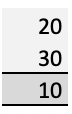
\includegraphics[scale=0.7]{screenshots/10_2030.png}
    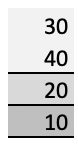
\includegraphics[scale=0.7]{screenshots/10_20_3040.png}
  \caption{Left: \texttt{\{10 [20 30]\}}. Right:  \texttt{\{10 \{20 [30 40]\}\}}.}
  \label{fig:format1}
\end{figure}

Note that backends  that do not have cell background colours will need to have different implementations for $\overleftarrow{\kappa}$. An example could be appending a dot for any $td > 1$, for example \verb|{10 {20 [30 40]}}| could be represented $30^{..}\; 40^{..}\;|\;20^{.}\;|\;10\;|$ without the appearance getting too ugly, I think.

\section{Direct products and spreadsheets}

Direct products of two grids lend themselves to being represented in two dimensions, since they can be naturally thought of as a rectangular grid. Remember that the direct product is referring to the \textit{grid} type, not the values. All the following examples are of grid type $\two \to P$: \verb|[10 20]|,  \verb|[30 40]|,  \verb|[50 60]|. The expression  \verb|[[10 20] [30 40] [50 60]]| is of type $\three \bigotimes \two \to P$ even though the inner values are different, you could replace the inner grids of type $\two \to P$ with any $P$. The key thing is that the inner grids are of the same type. They can be convoluted sum types, or a product type containing sum types (and so on and so forth...). 

\subsection{Products of sums}

For a direct product of sums, all the previous formatting rules can still apply if the product gets laid out horizontally, with sum types unfolding downwards. If $\gr{H}_n$ is a grid of sum type with length $n$, and $\gr{G}_m$ is a grid of the form $\bigoplus_m \unit$, then we employ the following rule:

\begin{equation} 
 \gr{G}_m \bigotimes \gr{H}_n \Rightarrow \mathbf{S}_{[n,m]} \label{eq:rule4}
\end{equation}

Examples of this rule, added to the previous rules, are given in Fig \ref{fig:format2}. 

\begin{figure}[h] 
\centering
  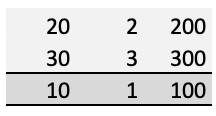
\includegraphics[scale=.7]{screenshots/prod1.png}
    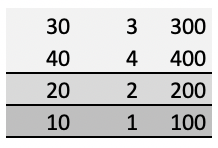
\includegraphics[scale=.7]{screenshots/prod2.png}
  \caption{Left: \texttt{[\{10 [20 30]\} \{1 [2 3]\} \{100 [200 300]\}]}. Right:  \texttt{[\{10 \{20 [30 40]\}\} \{1 \{2 [3 4]\}\} \{100 \{200 [300 400]\}\}]}.}
  \label{fig:format2}
\end{figure}

\subsection{Products of Products}




\end{document}
